\section{Data to the Cloud}
\label{sec:cloud}

There is a significant amount of data that is currently retained by
the controllers about water chemistry.  This includes historical
information on sensor readings (e.g., pH, oxidation-reduction potential (ORP),
free chlorine concentration, temperature, conductivity, turbidity,
alkalinity, etc.),
alarms (e.g., readings out of range, etc.), and user actions (e.g.,
set-point changes, etc.).
In addition, information on chemical stocks are frequently monitored
and logged as well.

It is currently possible to retrieve all of the above information from
a controller to a desktop application or mobile app by connecting to
the EZConnect server, providing appropriate authentication, and asking
the controller for its internal data logs.

Our current endeavor is
to collect this information off of a collection of controllers (e.g., all
owned by an individual organization), retain the collected data in
the cloud, and realize benefit from the aggregation that is not realized
from each individual controller's data in isolation.

Owner/operators of this equipment are responsible for 
more than one controller, and they would benefit significantly from a relevant
summary view of the state of the water chemistry under their purview.
An example of a summary view (appropriate for each controlled body of water)
is illustrated in Figure~\ref{screenshot}.

\begin{figure}[htbp]
 \center
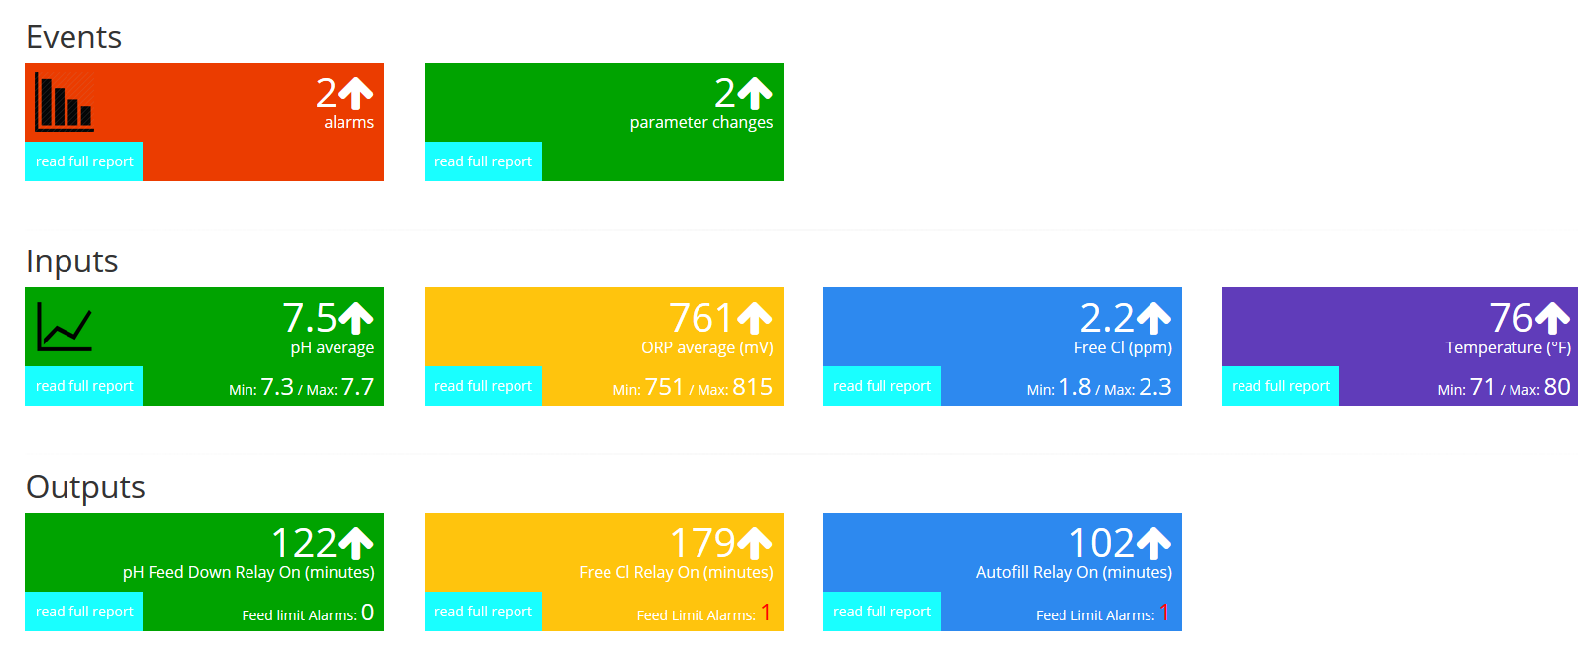
\includegraphics[width=\columnwidth]{screenshot}
    \caption{Screen capture of summary view data presentation. Additional
details are available via a link associated with each individual item.}
    \label{screenshot}
\end{figure}

In the figure, relevant information is organized for quick reference,
highlighting the ``big picture'' of the water chemistry, and allowing for
a more detailed drill down via a link associated with each item.
Groups of items are organized into categories (e.g., events, inputs,
outputs), and current values are supplemented with trends (indicated
by directional arrows) and ranges of values for the previous time period.

The above is facilitated by a number of concurrent processes running
in the EZConnect server (which is deployed in the cloud).  First,
a data logging process periodically communicates with each connected
controller and retrieves the data logs for that immediate past period.
Second, those data are inserted into a persistent database.  Third,
a report generator mines the database to generate the information needed
for the summary view, and finally, the summary view is served to the
user via a secure web server.
